\documentclass{beamer}
\usepackage[utf8]{inputenc}
\usepackage{amsmath, amsfonts, epsfig, xspace}
%\usepackage{algorithm,algorithmic}
\usepackage{pstricks,pst-node}
\usepackage{movie15} % multimedia, movie15
\usepackage[movieson]{optional}
\usepackage[normal,tight,center]{subfigure}
\usepackage{booktabs} % book-quality tables
\usepackage{fancybox}

\usepackage[utf8]{inputenc}
\usepackage{amssymb}

% PRESENTATION LANGUAGE
\usepackage[spanish]{babel}

% BIB
\usepackage{natbib}  
\def\newblock{}

% DEFINITION OF UPC BLUE
\definecolor{upcblue}{rgb}{0.262745098,0.556862745,0.77254902}
\definecolor{MainBlue}{rgb}{0.2,0.2,0.7}
\definecolor{MainGreen}{RGB}{0, 128, 0}
\definecolor{MainRed}{rgb}{0.73,0.08,0.21}
\definecolor{MyBrickRed}{rgb}{0.549, 0.239, 0.271}    
\definecolor{MyStrongRed}{rgb}{0.60, 0, 0.06}    
\definecolor{MyWebBrown}{rgb}{0.6, 0, 0}
\definecolor{MyWebBlue}{rgb}{0.2, 0.2, 1.0}%{0.07, 0.07, 0.53}

% http://en.wikibooks.org/wiki/LaTeX/Hyperlinks
% http://www.math.uakron.edu/~dpstory/tutorial/pdfmarks/hyper.pdf
\usepackage{hyperref} 
\hypersetup{colorlinks, urlcolor=MainBlue, citecolor=MainBlue, linkcolor=MainBlue} % BrickRed, RoyalBlue

% SUB-FIGURES
\setlength{\subfigcapskip}{-.5em}

% Beamer scheme
\usepackage{beamerthemesplit}
\usetheme{pdt}

% BASIC SCHEMES
%\usecolortheme[named=upcblue]{structure}
%\useinnertheme{rounded}
%\useoutertheme{shadow}

% SOME MINOR COLOR CHANGES
%\setbeamercolor{palette primary}{fg=upcblue,bg=white}
%\setbeamercolor{palette quaternary}{fg=white,bg=upcblue}

%% NEW COMMANDS
\newcommand{\Neurochem}{\textsc{NEUROChem} }
\newcommand{\Comedi}{\textsc{Comedi} }
\newcommand{\UPC}{Universitat Polit\`ecnica de Catalunya}

\newcommand{\R}{\texttt{R} }
\newcommand{\Python}{\texttt{Python} }

\newcommand{\smaller}{\tiny}
\newcommand{\mancite}[1]{{\scriptsize{\textbf{\color{MainGreen}{[#1] }}}}}

\renewcommand{\emph}[1]{{\color{MainBlue}{#1}}}


% GRAPHICS OPTIONS
\setkeys{Gin}{width=1.0\textwidth}
\graphicspath{{figures/}{images/}}

% INDENT
%\usepackage[parfill]{parskip}

% THE BASIC PRESENTATION INFORMATION
\title[\textnormal{Ph.D. Thesis Proposal \hspace{15em} \insertframenumber/\inserttotalframenumber}]{Computing Platform for Bioispired Chemical Gas Sensing}
\subtitle{Ph.D. Thesis Proposal}
\author[\textnormal{Andrey Ziyatdinov}]{Andrey Ziyatdinov}

%\institute{ 
%  { \small Advisor: Dr. Alexandre Perera} \\ \vspace{0.05\linewidth}  SISBIO - CREB - UPC}
\date{29 June, 2011}

% THE LOGO THAT WILL BE USED IN EACH PAGE
%\logo{
%\includegraphics[width=1.25cm]{logos/creb-upc.jpg} \insertframenumber/\inserttotalframenumber
%}

\begin{document}

% THE TITLE FRAME
\begin{frame}[plain]
  % THE HEADER WITH THE UPC AND CREB LOGOS
  \begin{center}
    \begin{tabular}[\textwidth]{lp{1cm}r}
      
\includegraphics[width=1.5cm]{logos/creb.jpg}
      &
      &
      
\includegraphics[width=1.5cm]{logos/upc.jpg}\\
      \texttt{\tiny Centre de Recerca en Enginyeria Biomèdica}
      &
      &
      \texttt{\tiny Universitat Politècnica de Catalunya}
    \end{tabular}
  \end{center}

  \begin{center}
    %\textsc{\LARGE University of Beer}\\[1.5cm]
    \textsc{\Large Ph.D. Thesis Proposal}\\[0.5cm]
    % Title
    %\HRule \\[0.4cm]
    {\huge \emph{Computing Platform for Bioispired Chemical Gas Sensing}}\\[0.4cm]
    %\HRule \\[1.5cm]

    % Author and supervisor
    \begin{minipage}{0.25\textwidth}
    \begin{flushleft} %\large
      Ph.D. Student: \\
      Supervisor: 
    \end{flushleft}
    \end{minipage}
    \begin{minipage}{0.6\textwidth}
    \begin{flushleft} %\large
      Andrey Ziyatdinov \\
      Alexandre Perera Lluna
    \end{flushleft}
    \end{minipage}
    
    \vfill

    % Bottom of the page
    {\large 29 June, 2011}
  \end{center}

  % THE REST OF THE TITLE
  %\maketitle
\end{frame}

\begin{frame}
  \frametitle{Outline}
  \tableofcontents
\end{frame}

% SECTION
\section{Introduction}

% SUB-ECTION
\subsection{Machine Olfaction}

% frame
\begin{frame}
\frametitle{A Story}
\begin{columns}
\column{0.6\textwidth}
The New York Times \\
\href{http://www.nytimes.com/2006/01/17/health/17dog.html}{Dogs Excel on Smell Test to Find Cancer} \\
{\scriptsize By Donald G. McNeil Jr., 2006}

\begin{block}{}
It has trained five dogs to detect lung cancer in the breath of cancer sufferers with 99\% accuracy. \\
{\scriptsize The Pine Street Clinic, CA}
% (tumors contain alkanes and benzene compounds)
\end{block}

Keys to success
\begin{itemize}
  \item Dogs detect odours in the very low parts-per-billion range
  \item The unique architecture of the olfactory pathway
\end{itemize}  

\column{0.4\textwidth}
\begin{center}
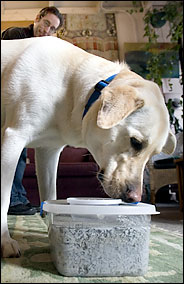
\includegraphics[width=.9\linewidth]{images/dog.jpg} \\
{\tiny Kobi in a cancer-detection experiment}
\end{center}
\end{columns}
\end{frame}

% frame
\begin{frame}
\frametitle{Machine Olfaction Device}
\begin{description}[leftmargin=0cm]
  \item[Definition:] Arrays of broadly-selective chemical sensors combined with a pattern recognition engine
  \item[Technologically:] A low-cost alternative to the instruments of analytical chemistry
  \item[Conceptually:] Attempt to mimic the olfactory system

\begin{center}
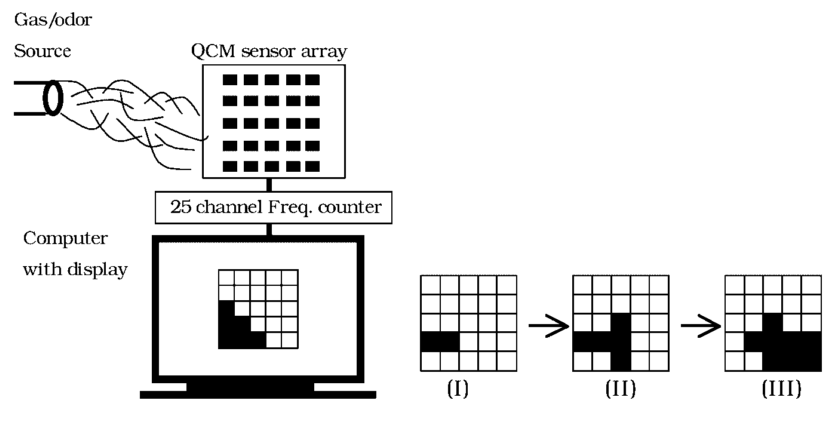
\includegraphics[width=.9\linewidth]{images/array-measurements-handbook.png} \\
\tiny{from \mancite{Pearce et al., 2003}}
\end{center}
\end{description}

\end{frame}

% SUB-ECTION
\subsection{State of the Art}

% frame
\begin{frame}
\frametitle{First Proposal}
\noindent First proposed by Persaud and Dodd in 1982
\begin{columns}
\column{0.7\textwidth}
\begin{block}{}
  ``... we suggest that to make fine
  discriminations between \emph{complex odorant mixtures} containing
  varying ratios of odorants without the necessity for highly
  specialized peripheral receptors, the olfactory systems makes
  use of feature detection using \emph{broadly tuned receptor cells}
  organized in a convergent neuron pathway. 
  %As a test of this
  %hypothesis we have constructed an \textcolor{blue}{electronic nose} using
  %semiconductor transducers and incorporating design features
  %suggested by our proposal
  ''
\end{block}
\column{0.3\textwidth}
\begin{center}
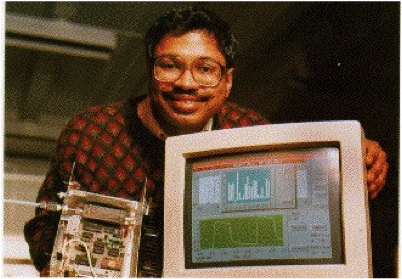
\includegraphics{images/krishna.png} \\
{\tiny Prof. K. Persaud and the e-nose}
\end{center}
\end{columns}
\end{frame}

% frame
\begin{frame}
\frametitle{State of the Art}
\begin{itemize}
  \item Sensor Array Technology
  \item Data Processing
  \item Findings in Biology 
\end{itemize}
\end{frame}

% frame
\begin{frame}
\frametitle{Sensor Array Technology}
\begin{center}
\includegraphics[width=0.7\linewidth]{sensor-technology.png} \\
{\tiny 
(a) Metal Oxide; (b) Quartz Crystal Microbalance; \\
(c) Surface Acoustic Waves; (d) Optical fiber \\
from \mancite{Gutierrez-Osuna, 1998} 
}
\end{center}
\end{frame}


% frame
\begin{frame}
\frametitle{Data Processing}
\begin{center}
\includegraphics[width=1.0\linewidth]{images/data-processing.png} \\
{\tiny from \mancite{Gutierrez-Osuna, 2002}}

\begin{itemize}
  \item Low-dimensional input data
  \item Transient feature extraction
  \item Testing Datasets
  \item Standardize evaluation of the algorithms (benchmarking)
\end{itemize}  

\end{center}
\end{frame}

% frame
\begin{frame}
\frametitle{Data Processing}
\begin{columns}
\column{0.5\textwidth}
Review on signal processing for sensor arrays
\begin{itemize}
  \item \mancite{Gutierrez-Osuna, 2002}
  \item \mancite{Pearce et al., 2003}
  \item \mancite{Martinez et al., 2008}  
\end{itemize}  
\column{0.5\textwidth}
\begin{center}
\includegraphics[width=1.0\linewidth]{images/methods.png} \\
{\tiny from \mancite{Raman, 2005}}
\end{center}
\end{columns}
\end{frame}

% frame
\begin{frame}
\frametitle{Findings in Biology}
\begin{columns}
\column{0.5\textwidth}
\includegraphics[width=1.0\linewidth]{images/olfactory-pathway.png} 
\column{0.5\textwidth}
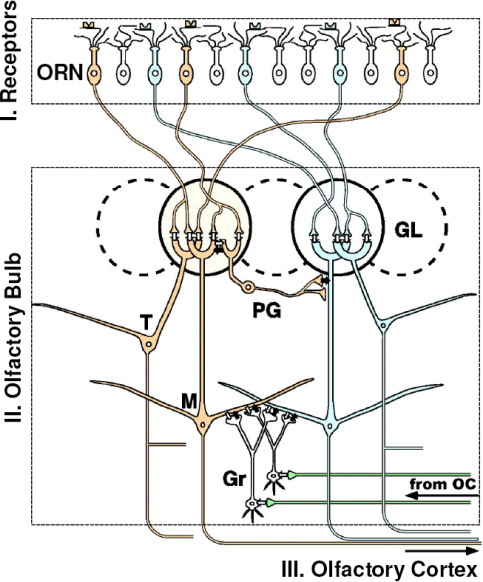
\includegraphics[width=1.0\linewidth]{images/olf-pathway-scheme.png}
\end{columns}
\end{frame}

% frame
\begin{frame}
\frametitle{Findings in Biology}
\begin{columns}
\column{0.5\textwidth}
Milestones
\begin{itemize}
  \item Seven trans-membrane proteins %mediate the chemical-electrical transduction through ORNs
  \mancite{Axel and Buck, 1991, Nobel Prize}
  \item ORNs respond to odotopes %odourant molecular features % e.g. carbon-change length, benzene rings, etc
  \mancite{Shepherd, 1987, 1994}
  \item Ordered convergence to glomeruli % ordered projection of ORN into spherical regions (
  \mancite{Vassar, 1994}
  \item Inhibitory connections to improve odour recognition % odour representation through          
  \mancite{Wilson, 2004}
\end{itemize}
\column{0.5\textwidth}
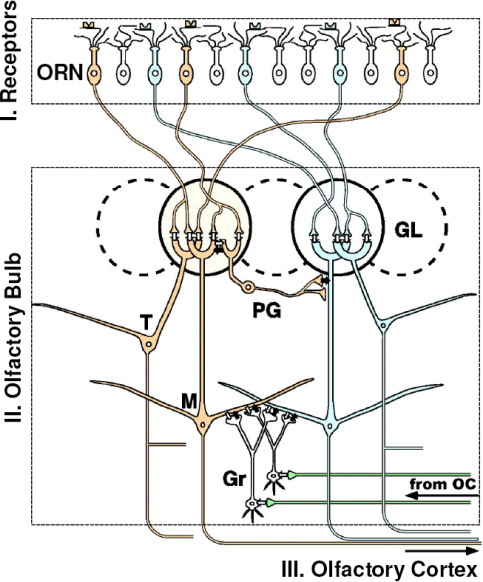
\includegraphics[width=1.0\linewidth]{images/olf-pathway-scheme.png}
\end{columns}
\end{frame}

\begin{frame}
\frametitle{Bioinspired Data Processing}
Neuromorphic models
\begin{itemize}
  \item Habituation to odour mixture \mancite{Gutierrez-Osuna, 2005}
  \item Convergence to GL (via SOM) \mancite{Raman and Gutierrez-Osuna, 2006}
  \item Dimensionality-reduction technique inspired by ORN convergence \mancite {Perera, 2006}
  \item OB circuitry in silicon \mancite{Pearce, 2005}
\end{itemize}
    
Receptor Systems
\begin{itemize}
  \item Topology of ORN population \mancite{Gill and Pearce, 2005}
  \item Current sensor arrays have an extremely low number of sensing elements \mancite{Gardner, 2006}
\end{itemize}
\end{frame}

% SECTION
\section{Motivation}

% SUB-ECTION
\subsection{Computing Platform}


\begin{frame}
  \frametitle{Motivation}
\begin{block}{}
     \begin{columns}
   \column{0.6\textwidth}
   European research project (2008-2011)\\
   In Bio-ICT Convergence\\
   7$^{th}$FP

   \column{0.4\textwidth}
      \includegraphics[width=0.5\textwidth]{logos/neurochem_logo.png} \\
      \tiny{\href{http://www.neurochem-project.org/}{http://www.neurochem-project.org/}} \\
      \tiny{\href{http://neurochem.sisbio.recerca.upc.edu/}{http://neurochem.sisbio.recerca.upc.edu/}}
    \end{columns}
    \end{block}
 \begin{block}{NEUROChem Goals}

      \begin{itemize}
        \item Explore novel computing paradigms.
%The first goal addressed by the project is to explore novel computing paradigms
%based on the information representation and processing of the olfactory path-
%way to overcome existent problems in chemical sensing. Particularly, the key
%points for investigation include early encoding of chemical information, ORN
%redundancy, odour segmentation odour memory and odour response decorrelation.        
        \item Build biomimetic artifacts.
% As a direct application of the novel computing paradigms extracted, the second
%project goal is to build biomimetic artifacts that will be able to perform chemical
%sensing. Constructing a chemical sensor array with this huge amount of sensors
%(approaching 106 ORN in the mammalian olfactory system) will be hosted on
%the embedded system on the mobile platform.

          \item  Demonstrate the biomimetic device on mobile platform 
      hosting the 64K sensor array and real-time processing and visualization.

      \end{itemize}
    \end{block}

%    \begin{block}{Stages}
%     \begin{itemize}
%        \item set up computing platform
%        \item run bioinspired models
%     \end{itemize}
%    \end{block}

 \end{frame}
 
% SECTION
\section{Goals}

% SUB-ECTION
\subsection{Expected Contributions}

% frame
\begin{frame}
\frametitle{Goals (I)}
\begin{description}
  \item[Platform:] Design of computing platform based on an embedded computer.
  \item[Datasets:] Acquisition and characterization of datasets from MOX, conducting polymer and synthetic sensors.  
  \item[Data Processing:] Compensate noise and drift artifacts, explore proper pattern recognition tools.
  \item[Benchmarking:] Create benchmarking datasets as scenarios with programmed level of difficulty.    
\end{description}
\end{frame}

% frame
\begin{frame}
\frametitle{Goals (II)}
\begin{description} 
  \item[Virtual Array:] Build a device simulator of very large sensor array.  
  \item[Virtual Platform:] Virtualize the proposed platform for the synthetic experiments.  
  \item[Robotic Experiments:] Test the mobile robot on the task of odour source localization.
  \item[Bioinspired Algorithms:] Focus on processing a high-dimensional input.  
\end{description}
\end{frame}

% frame
\begin{frame}
\frametitle{Expected Contribution}
\begin{description} 
  \item[Machine Olfaction Device:] Autonomous mobile computing platform featured with the large-scale sensor array (possibly the largest).
  \item[Synthetic Experiments:] A set of benchmarks (not established in the field).
  \item[Virtual Image:] An educational tool with complete set of utilities.
  \item[Open Software:] To make the published results available and reproducible.
\end{description}
\end{frame}

% SECTION
\section{Methodology}

% frame
\begin{frame}
\frametitle{Methodology}
\begin{itemize}
  \item Computing Platform
  \item Drift Compensation
  \item Synthetic Sensor Array
  \item Benchmarks
  \item Software Output
\end{itemize}
\end{frame}

% SUB-ECTION
\subsection{Computing Platform}

% frame
\begin{frame}
\frametitle{Computing Platform}
\begin{center}
\includegraphics[width=1.0\linewidth]{images/neurochem-platform.png} \\
\end{center}
\end{frame}

\begin{frame}
  \frametitle{Platform Features}
  \begin{columns}
    \column{0.45\textwidth}  
    \centering \includegraphics[width=1.0\textwidth]{neurochem-embedded.pdf}
    
    \column{0.65\textwidth}  
    {\small 
    \begin{block}{Interfaces}
      \begin{itemize}
      \item Sensor Array   {\tiny (power, configuration, acquisition)}
      \item Mobile Platform   {\tiny (bluetooth com, USB joystick, ultrasonic sensors,
          compass, accelerometer, GPS, wind vane)}
      \item Gas Station 
     \end{itemize}   
    \end{block}
    \begin{block}{Features}
      \begin{itemize}
      \item Compact size  {\tiny (4 boards in stack)}
      \item Reasonable power consumption  {\tiny (10W SA + 15W Embedded)}
      \item Autonomous 1.1h 
      \end{itemize} 
    \end{block} 
} %small
  \end{columns}
\end{frame}

\begin{frame}
  \frametitle{Platform Assembled}

  \begin{center}
    \includegraphics[width=0.8\textwidth]{Embedded-SA-Monitor.JPG}
  \end{center}
\end{frame}

% SUB-ECTION
\subsection{Drift Compensation}

% frame
\begin{frame}
\frametitle{Drift Problem}
\begin{columns}
  \column{0.70\textwidth}
\begin{description}%[leftmargin=0cm]
  \item[Definition] Gradual changes in a quantitative characteristic 
  that is assumed to be constant over time
  \item [Sensors] Complex and inevitable effect which is generated by different sources
%  \begin{itemize}
%    \item sensor aging, sensor poisoning, experimental operation, environment
%  \end{itemize}
\end{description}
  \column{0.30\textwidth}
  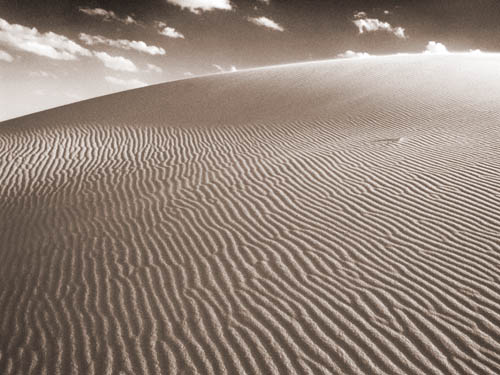
\includegraphics[width=0.9\textwidth]{images/wind-sand-sky.jpg} 
\end{columns}

\begin{center}
\begin{columns}
  \column{0.50\textwidth}
  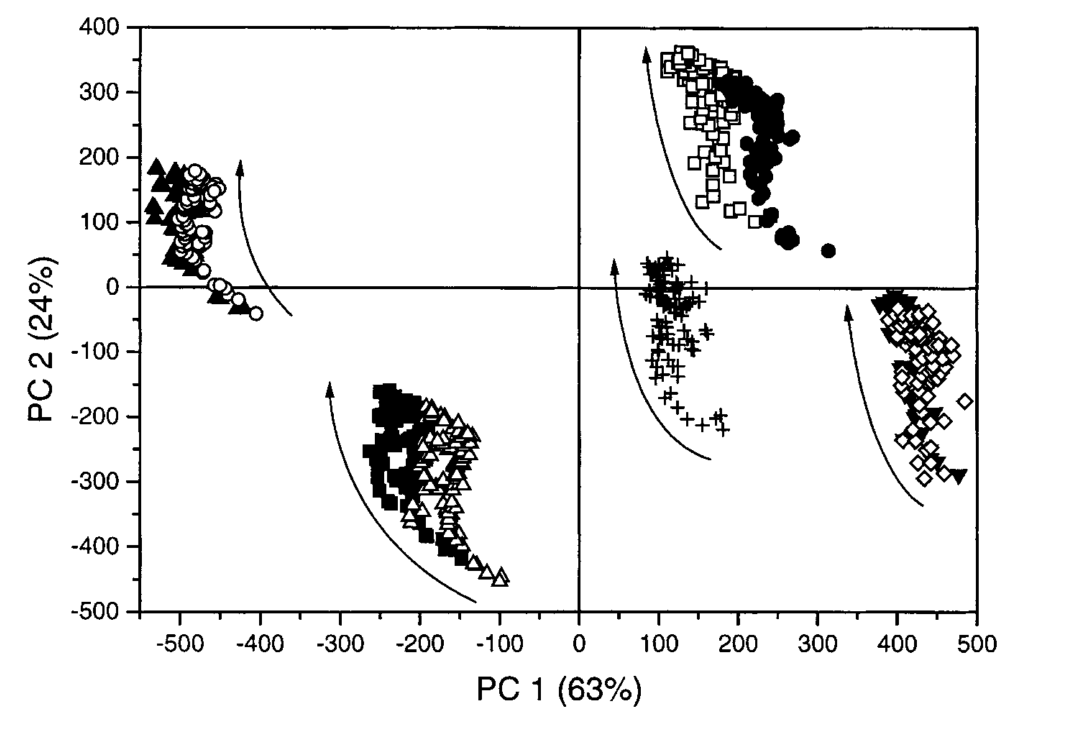
\includegraphics[width=0.9\textwidth]{images/mvar-drift-1.png}
  \column{0.50\textwidth}
  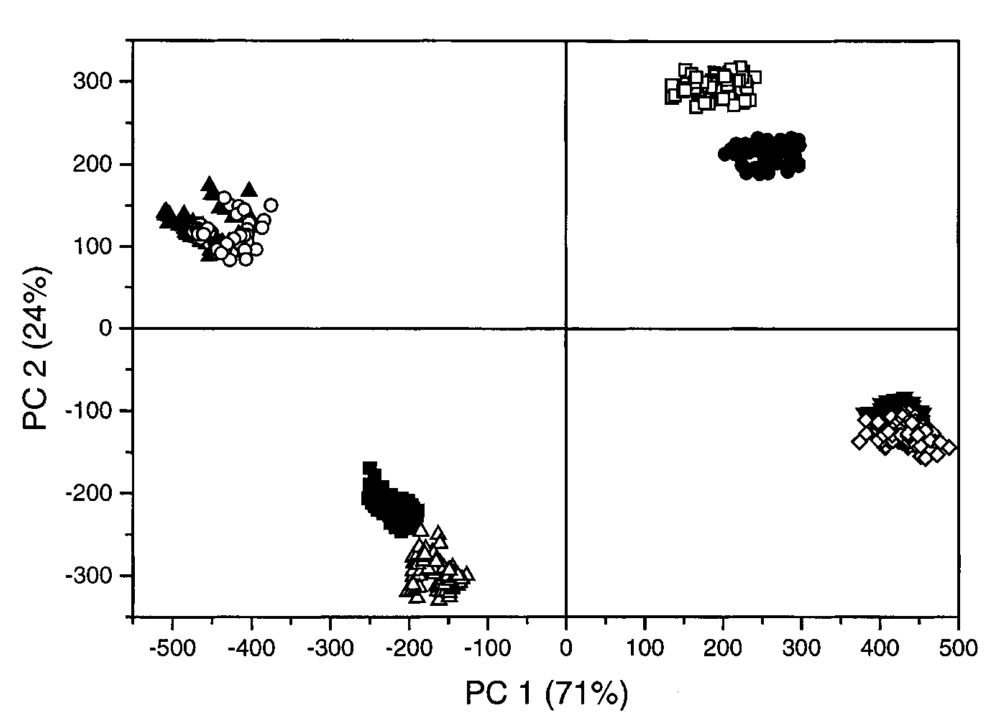
\includegraphics[width=0.9\textwidth]{images/mvar-drift-2.png}
\end{columns}
{\tiny from \mancite{Artursson, 2002}}
%{\tiny from [Gründler, 2008] }
\end{center}
\end{frame}

% frame
\begin{frame}
\frametitle{Common PCA}
\begin{description}
  \item[Idea] Drift is a variance component common to all classes
  \item[Method] Joint diagonalization of covariance matricies
\end{description}

\begin{equation*}
  V' \cdot 
  \begin{pmatrix} \Sigma_{1} \\ \Sigma_{2} \\ \Sigma_{3} \end{pmatrix} \cdot
  V = 
  \begin{pmatrix} \Lambda_{1} \\ \Lambda_{2} \\ \Lambda_{3} \end{pmatrix}
\end{equation*}

\begin{columns}
  \column{0.30\textwidth}
  \includegraphics[width=0.9\textwidth]{images/cpca-0.png}
  \column{0.30\textwidth}
  \includegraphics[width=0.9\textwidth]{images/cpca-2.png}
  \column{0.30\textwidth}
  \includegraphics[width=0.9\textwidth]{images/cpca-3.png}
\end{columns} 
  
\end{frame}

% frame
\begin{frame}
\frametitle{Numerical Results}
Novel method for drift compensation \mancite{Ziyatdinov et al., 2010}
\begin{itemize}
  \item 3 gases, $\sim$4000 samples
  \item common drift space of one component
  \item evaluation by k-NN classifier 
\end{itemize}

\begin{center}
  \includegraphics[width=0.7\textwidth]{images/cpca-results.png}
\end{center}
\end{frame}

  
% SUB-ECTION
\subsection{Virtual Sensor Array}


\begin{frame}
  \frametitle{Virtual Sensor Array}
   \begin{columns}
    \column{0.55\textwidth}
    Sensor Device Model
      \begin{itemize}
        \item Any number of sensors
        \item Any gas mixture
        \item Noise control (type, strength)
      \end{itemize}    
    \column{0.45\textwidth}
    %\includegraphics[width=0.3\textwidth]{conc-noise.pdf}
    %\includegraphics[width=0.3\textwidth]{sa-drift.png}
    %\includegraphics[width=0.3\textwidth]{mixture-model.pdf}        
  \end{columns}  
  
  \begin{columns}
    \column{0.45\textwidth}
    \includegraphics[width=0.9\textwidth]{images/scneario.pdf} \\
    {\tiny 20 samples} \\
    \column{0.45\textwidth}
    \includegraphics[width=0.9\textwidth]{images/sdata-10.pdf} \\
    {\tiny 20 samples x 10 sensors} \\
   % \column{0.33\textwidth}
    %\includegraphics[width=1.0\textwidth]{sdata-100.pdf} \\
    %{\tiny 20 samples x 100 sensors} \\
  \end{columns}  
\end{frame}

\begin{frame}
\frametitle{Synthetic Sensors}
1000 sensors and two gases
\begin{center}
  % 640x440, ratio 1.3
  %\includegraphics[width=0.5\textwidth]{videos/robot-nav-2-sources.png}
  \includemovie[poster, autoplay]{7cm}{7cm}{videos/sensors.avi}   
 \end{center}
\end{frame}

\begin{frame}
\frametitle{Synthetic Experiments}
Integration into IQR neural simulator
\begin{center}
  % 640x440, ratio 1.3
  %\includegraphics[width=0.5\textwidth]{videos/robot-nav-2-sources.png}
  \includemovie[poster, autoplay]{7cm}{7cm}{videos/iqr-demo.avi}   
 \end{center}
\end{frame}

\begin{frame}
  \frametitle{Virtual'em all}
 
  \begin{center}
    \includegraphics[width=1.0\textwidth]{NCimage}
  \end{center}
 \end{frame}

\section{Conclusions}

\subsection{Workplan}

\begin{frame}
\frametitle{Workplan}
\begin{center}
  \includegraphics[width=1.0\textwidth]{images/workplan.png}
 \end{center}
\end{frame}

\begin{frame}
\frametitle{Final Robot Video}
\begin{center}
  % 640x440, ratio 1.3
  %\includegraphics[width=0.5\textwidth]{videos/robot-nav-2-sources.png}
  \includemovie[poster, autoplay]{6.4cm}{4.8cm}{videos/robot-nav-2-sources.avi}   
 \end{center}
\end{frame}

\begin{frame}
\frametitle{Thank you}
\begin{center}
  {\Large Thank you for your attention!}
 \end{center}
\end{frame}

\bibliography{pdt}

\end{document}



